\section{JET SUPPRESSION}
\label{jets}
Unlike the production of electroweak bosons, which is observed to be essentially described by
an independent superposition of nucleon-nucleon collisions within current experimental uncertainties,
jet production is substantially modified in high energy heavy ion collisions.
%The first indications of this were observed by all four major experiments at the RHIC collider.
%The rates of high transverse momentum ($\pT>4$ GeV) particles emitted in Au+Au collisions
%were found to be suppressed
%by a factor of approximately 5 relative to the rates predicted using the number of binary
%collisions, something not seen in d+Au collisions (ruling out strong nPDF effects).
%Correlations of high momentum particle pairs (typically referred to as ``trigger'' and ``associated''
%particles) also showed a distinctive signature of the disappearance
%of back-to-back associated particle emission in Au+Au up to trigger $\pT \sim 8$ GeV, 
%again something not observed in d+Au.
The RHIC experimental program did not have the large acceptance detectors or the large jet rates 
available at the LHC, and so jet measurements have been particularly challenging and no 
published results are available.
Jets are measured by all three large LHC experiments.  ATLAS and CMS are similar in that they
have large acceptance ($|\eta|<5$) hadronic and electromagnetic calorimetric coverage, and 
precise silicon trackers ($|\eta|<2.4$ for CMS and $|\eta|<2.5$ for ATLAS), 
both of which are used in jet measurements.
%ATLAS primarily relies on calorimetric jet measurements, grouping smaller readout ``cells''
%into towers of angular size $\Delta \eta \times \Delta \phi = 0.1 \times 0.1$. 
%The anti-$k_t$ jet clustering algorithm is used to partition the towers into proto-jets
%and exclude towers in regions with large localized energy depositions.  The remaining towers
%are then used to estimate the uncorrelated background as a function of $\eta$, including
%an estimate for an overall azimuthal modulation due to elliptic flow.  This background is subtracted
%cell-by-cell in each calorimeter 
%layer from all remaining jet candidates and then the background estimated again after excluding
%jets with $E_T>25$ GeV.  After this second step the background is subtracted again from all
%jets, and the final jet kinematics are recalculated using the subtracted cells.
%CMS also uses an iterative procedure based on calorimeter towers.  For each $\eta$ ring
%of $\Delta \eta \sim 0.87$, the average transverse energy and standard deviation are calculated
%for each event and $\langle E_T \rangle + \sigma$ are subtracted from each event, and negative
%values are set to zero.  Jets are then found using an iterative cone algorithm, the tower background
%recalculated after excluding jets of at least 30 GeV, and the final jets are reconstructed 
%on the subtracted towers.
ATLAS primarily relies on calorimetric jet measurement, grouping smaller readout ``cells''      
into towers of angular size $\Delta \eta \times \Delta \phi = 0.1 \times 0.1$, and 
clustering them with the anti-$k_t$ algorithm with varying cone size.
CMS uses both a seeded cone algorithm and a 
particle flow technique, providing tracks and calorimeter objects to the 
anti-$k_t$ algorithm with $R=0.3$.
ALICE has much smaller angular coverage and so no published full jet results are available.

\subsection{Dijet correlations}

The first result on jets at the LHC was released by the ATLAS collaboration 
several weeks after first collisions were seen by the three main experiments.  
ATLAS performed a measurement~\cite{Aad:2010bu} of
the asymmetry between the two highest-energy jets in events with at least one jet
with $E_{T1} > 100$ GeV, and a second jet $E_{T2} > 25$ GeV.  The asymmetry is
then defined as $A_J = (E_{T1} - E_{T2})/(E_{T1} + E_{T2})$.
Figure~\ref{fig:pas:final_4x2} shows the evolution of the distribution of
$A_J$ with collision centrality, compared to both proton-proton data at 7 TeV
as well as a full simulation of events where PYTHIA dijets are embedded into
Pb+Pb events generated by HIJING.
It is observed that while the distributions in the 40-80\% most central events
resemble the simulated events and the pp data, the $A_J$ distribution becomes
progressively wider in the more central events, indicating an increasing attenuation
of the energy of the second jet relative to the leading jet.  This is generally
understood to be a direct observation of jet quenching, where the jet loses energy
in the hot and dense medium.
%While the RHIC results generated a wide range of theoretical descriptions, the reliance
%on leading particles precluded strong statements about the nature of the energy
%loss process, whether it was from the inducement of a single hard radiative gluon
%from the primary, or from many soft radiations.
The lower row on the ATLAS figure already indicated that the energy loss could not be
from single hard emissions since the back-to-back pattern observed in pp and in
the most peripheral sample was essentially unchanged even in the 0-10\% most
central events.

\begin{figure}[!thb]
\begin{center}
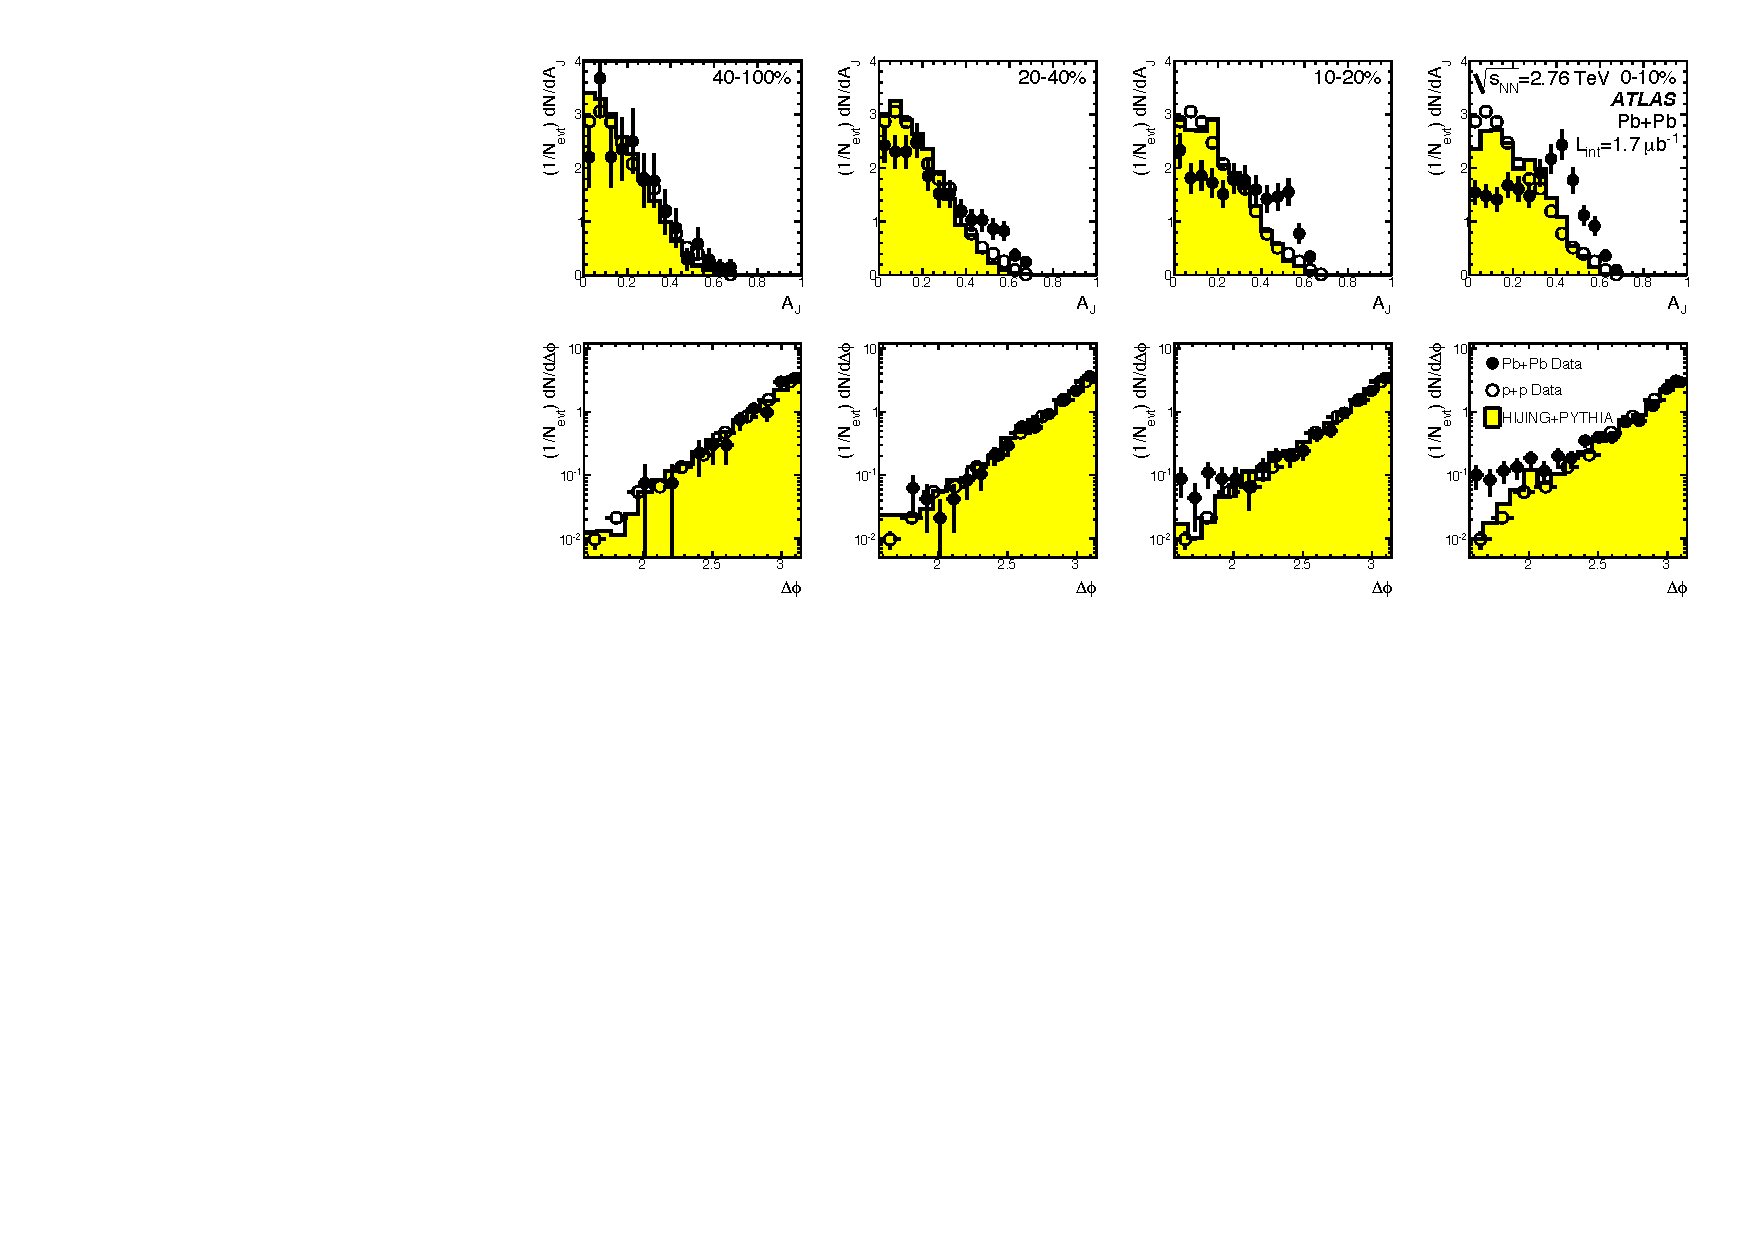
\includegraphics[width=0.8\textwidth]{jetfigures/final_4x2_23_newpp.pdf}
\caption{
(top) Dijet asymmetry distributions for data (points) and {\sc{hijing+pythia}} 
simulations (solid yellow histograms), as a function of collision centrality.  
Proton-proton data from $\sqrt{s}=7$\TeV\ is shown as open circles.
(bottom) Distribution of $\dphi$ between the two jets, 
for data and {\sc{hijing+pythia}}, shown in four bins of centrality.
Reproduced from~\cite{Aad:2010bu}.
}
\label{fig:pas:final_4x2}
\end{center}
\end{figure}

CMS extended this study using the higher-statistics 2011 Pb+Pb dataset~\cite{CMS_dijet} 
(with nearly a
factor of 100 increase in luminosity relative to the original ATLAS paper).
%Their result shows the evolution of $\langle p_{T,2}/p_{T,1} \rangle$, 
%using events with jet $p_{T1} > 120$ GeV, jet $p_{T,2} > 30$ GeV
%and $\Delta\phi_{12} > 2\pi/3$ to select back-to-back topologies, is shown in Figure~\ref{fig:PAS:CMS_pt_ratio}
%as a function of $p_{T,1}$.
%Since these data do not unfold the effect of the known experimental energy resolution for jets,
%they are compared to similarly reconstructed pp data as well as fully-reconstructed HYDJET events
%with embedded PYTHIA dijets.
%The rising trend observed in each panel, both the heavy ion and pp data, as well as the simulated events,
%can be generally understood as arising from the $\pT$ dependence of the jet resolution, which degrades at lower
%jet $\pT$, and thus pushes the reconstructed $\langle p_{T,2}/p_{T,1} \rangle$ lower simply from the 
%ordering of the jets.
%However, the difference between data and simulation increases significantly as the events become more
%central.  This is shown in the lower panels as a function of $p_{T,1}$ and is found to be constant within
%experimental uncertainties.

%\begin{figure}[!th]
%\begin{center}
%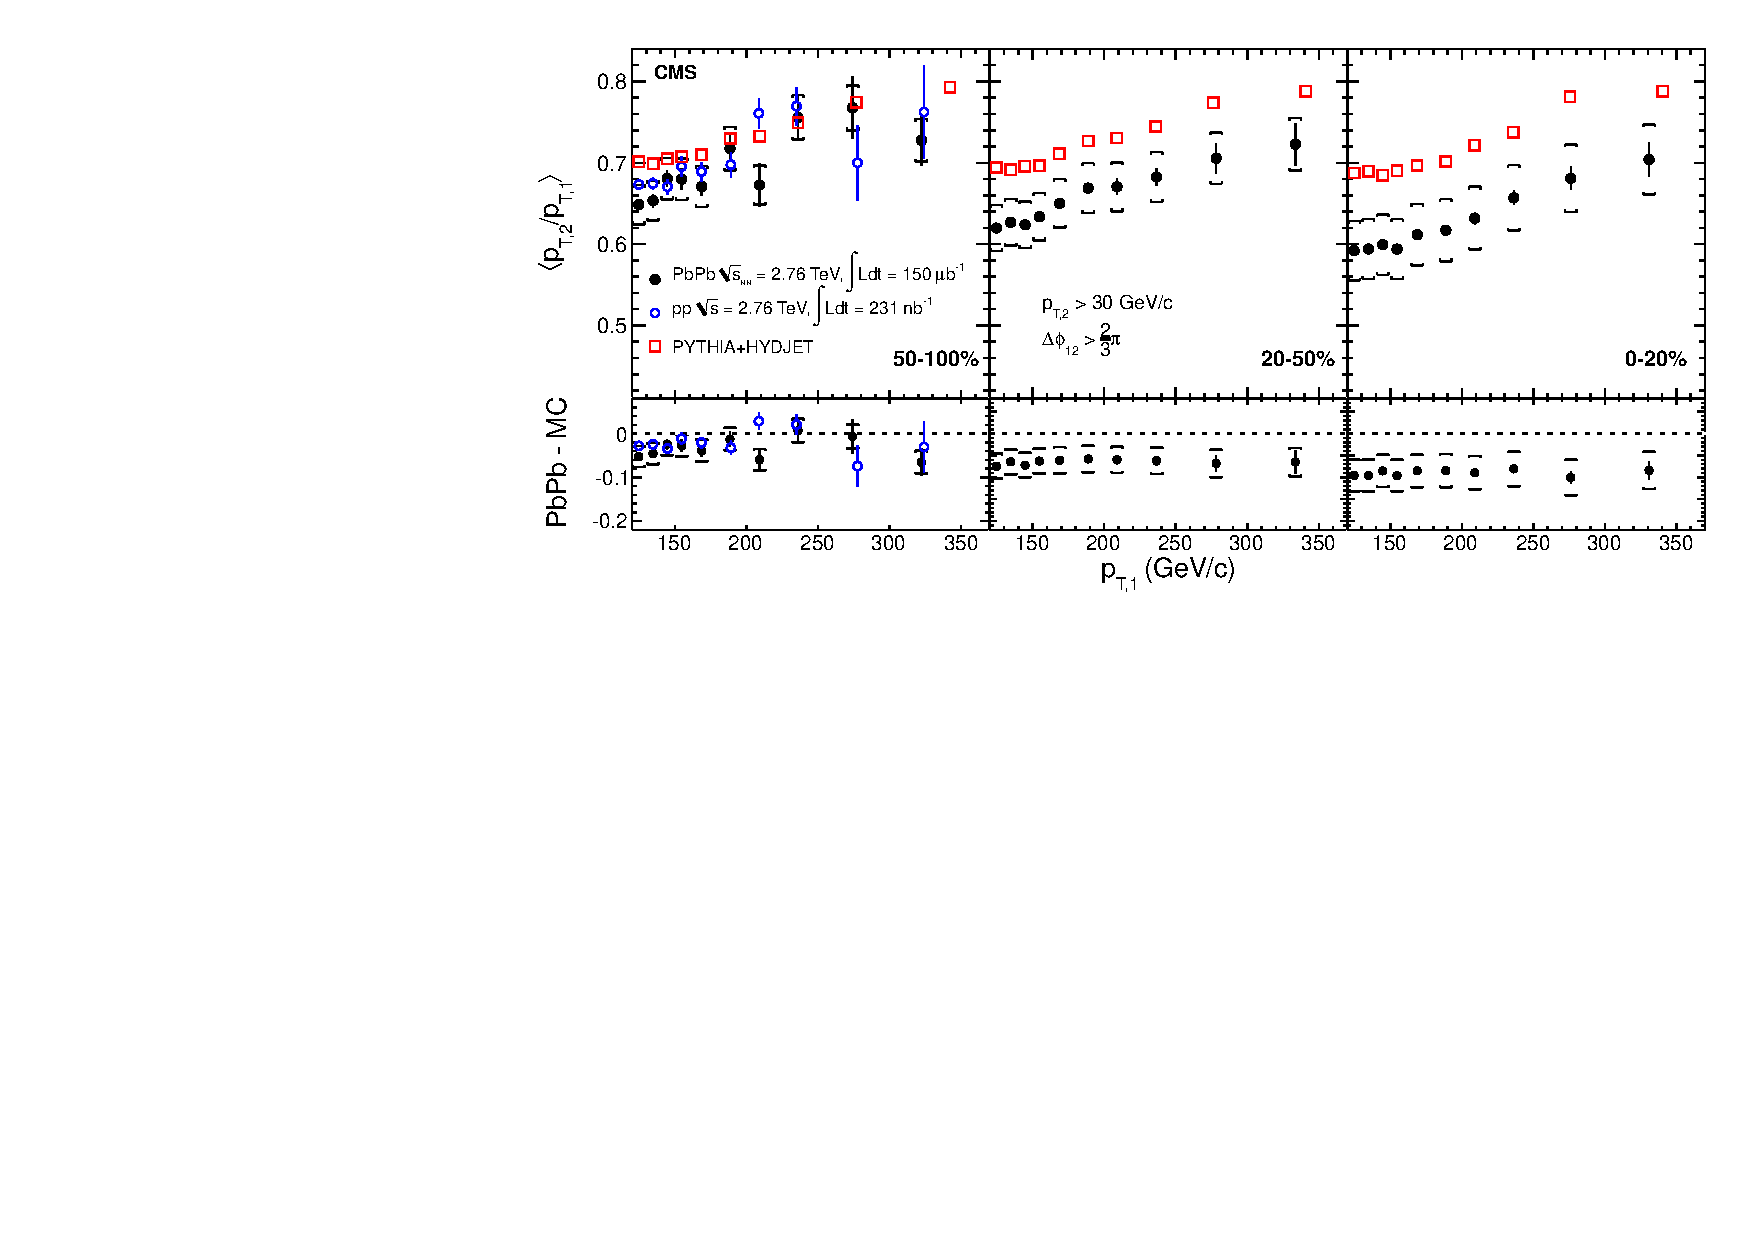
\includegraphics[width=0.75\textwidth]{jetfigures/deltaPtOverPt5_lead120_sub30_diff_20120103.pdf}
%%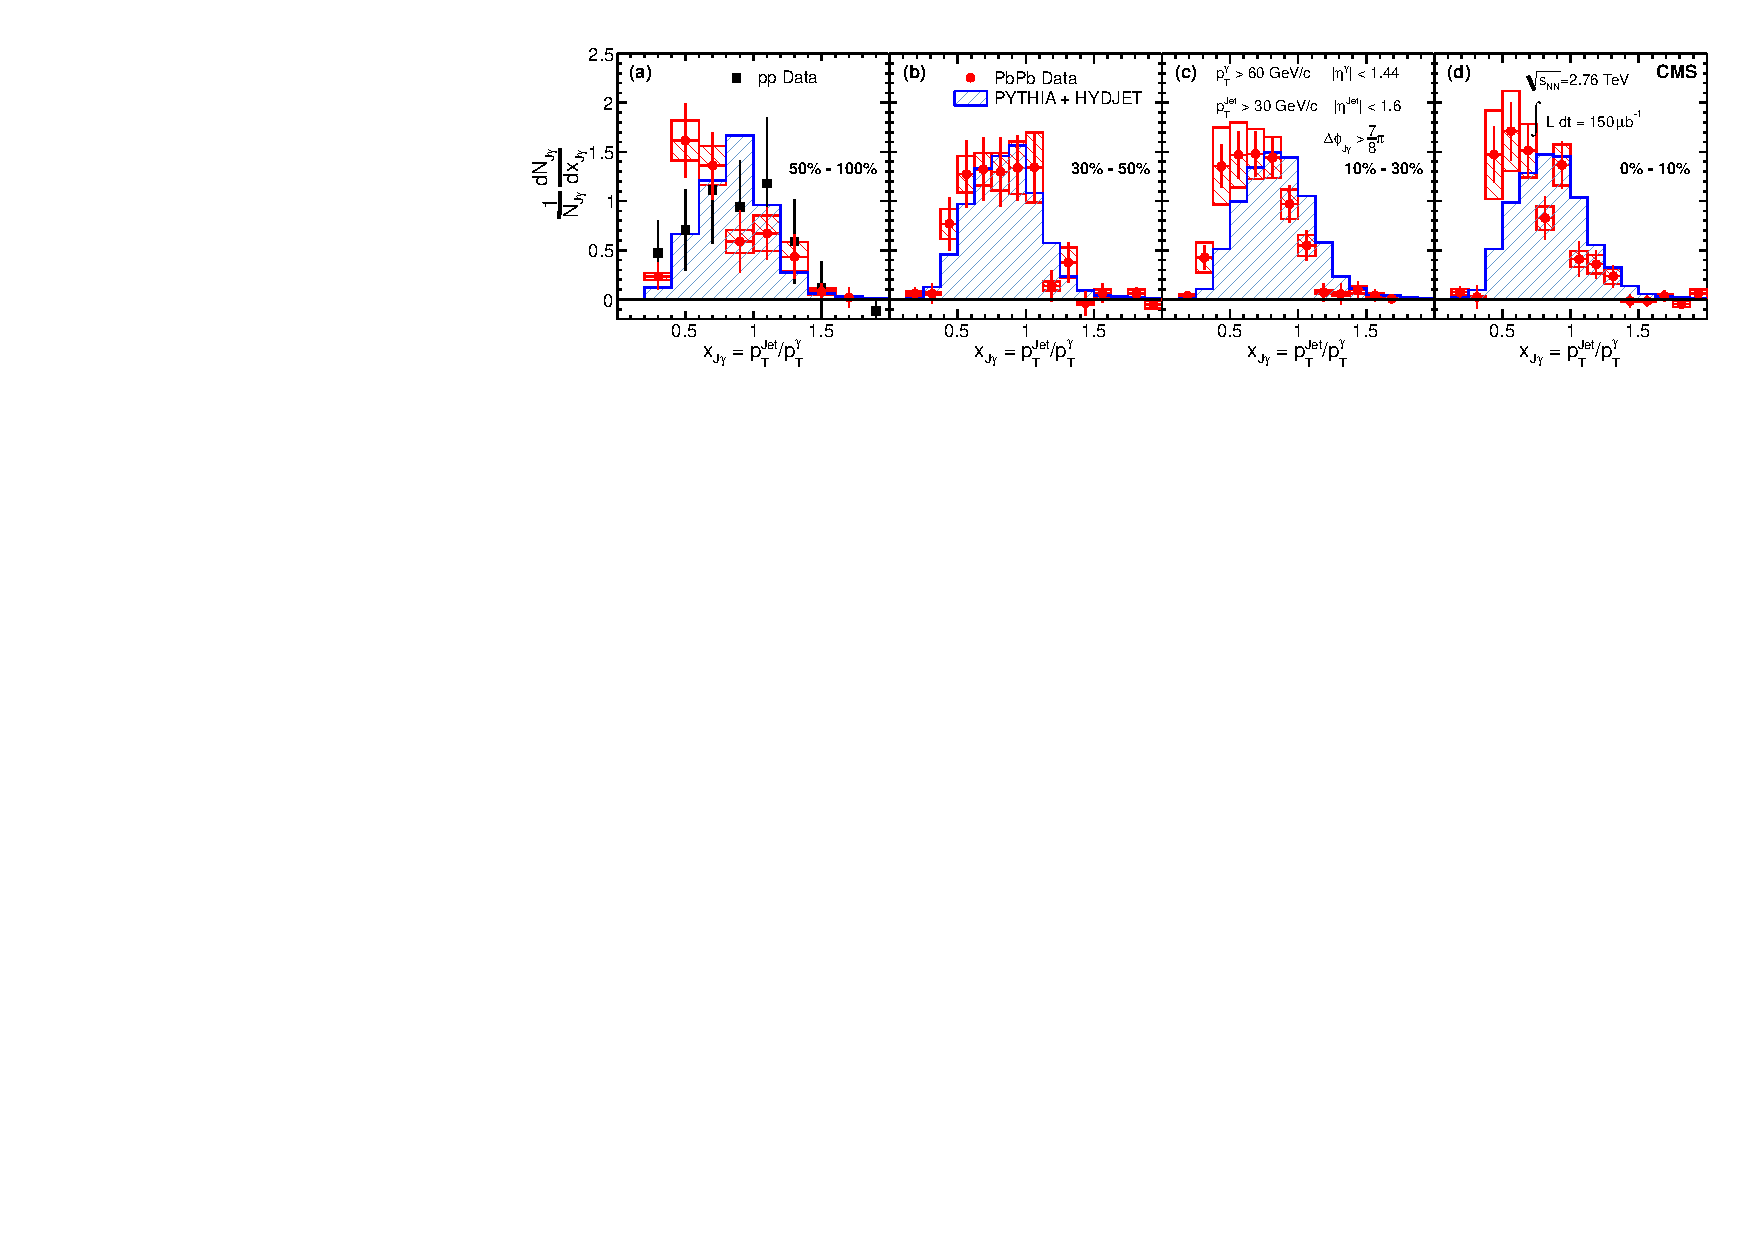
\includegraphics[width=0.75\textwidth]{jetfigures/Photonv7_Paper_InclPtRatio_all_cent4_G60J30_subDPhi1SS1_Isol0_Norm1log1.pdf}
%\caption{
%(top, upper): Dijet momentum ratio $\langle \ptsub/\ptlead \rangle$ as a function of
%leading jet \pT\ in three bins of collision centrality.
%\PbPb\ data are shown as points, with brackets indicating systematic uncertainties.  
%\PYTHYD\ calculations are shown as squares. In the peripheral bin,
%\pp\ data are displayed as open circles.
%(top, lower): Difference of $\langle \ptsub/\ptlead \rangle$ between the \PbPb\ results and \PYTHYD\ reference.
%Reproduced from~\cite{CMS_dijet}.
%(bottom)
%Distribution of the photon/jet 
%momentum ratio, \xjg, in four bins of collision centrality. 
%  The distributions are normalised to unit area. All panels compare
%\PbPb\ data (filled circles) to \pp\ data at
%  2.76\TeV\ (filled squares), and to the \PYTHYD\ MC simulations
%  (shaded histogram). Error bars show the statistical uncertainties and
%boxes show the (anti-correlated) systematic uncertainties. Reproduced from~\cite{Chatrchyan:2012gt}.
%}
%\label{fig:PAS:CMS_pt_ratio}
%\end{center}
%\end{figure}


\subsection{Jet yields and jet suppression}

While the dijet correlations were effective at demonstrating the presence of jet energy loss, 
they are in principle limited in their sensitivity to jet quenching physics by the fact that
there is no control over the energy loss of the leading jet.
This is certainly mitigated by the use of electroweak bosons in place of the leading jet,
for which initial CMS data exists but with relatively low statistics.
A more direct means to access the physics of energy loss is with the suppression of single
jet yields relative to a sample in which one expects energy loss effects to be minimal.
Both proton-proton collisions and peripheral heavy ion events are both used as the reference,
the latter in principle including nPDF and isospin effects which are absent in pp.

The left panel of Figure~\ref{fig:pas:rcprfour} shows the suppression of jets in Pb+Pb
in central events relative to peripheral via the ratio $R_{CP}$
\begin{equation}
R_{CP} = \frac{dN_{C}/d\pT / N_{coll,C}} {dN_{P}/d\pT / N_{coll,P}}
\end{equation}
where $C$ indicates the 0-10\% most central events and $P$ indicates the 60-80\% centrality interval.
For a given jet radius (e.g. $R=0.4$ shown here), no signficant $\pT$ dependence is observed.
However, as the centrality is increased, the yield of jets becomes systematically more suppressed,
reaching approximately a factor of two suppresison in the 0-10\% centrality interval.

Within a given centrality interval, the study of jet rates as a function their angle relative 
to the event plane provides a means to study the path length dependence of jet quenching.
The right panel of Figure~\ref{fig:pas:rcprfour} shows measured values of $v_2$ as a function
of jet $\pT$, where $v_2$ is the amplitude of an observed $\cos(2\phi)$ modulation relative to
the event plane measued with the ATLAS forward calorimeters.  This ``elliptic'' modulation of
jet rates has already provided similar information as high $\pT$ hadrons, but without 
any effects from the non-perturbative jet fragmentation functions.

\begin{figure}[!th]
\begin{center}
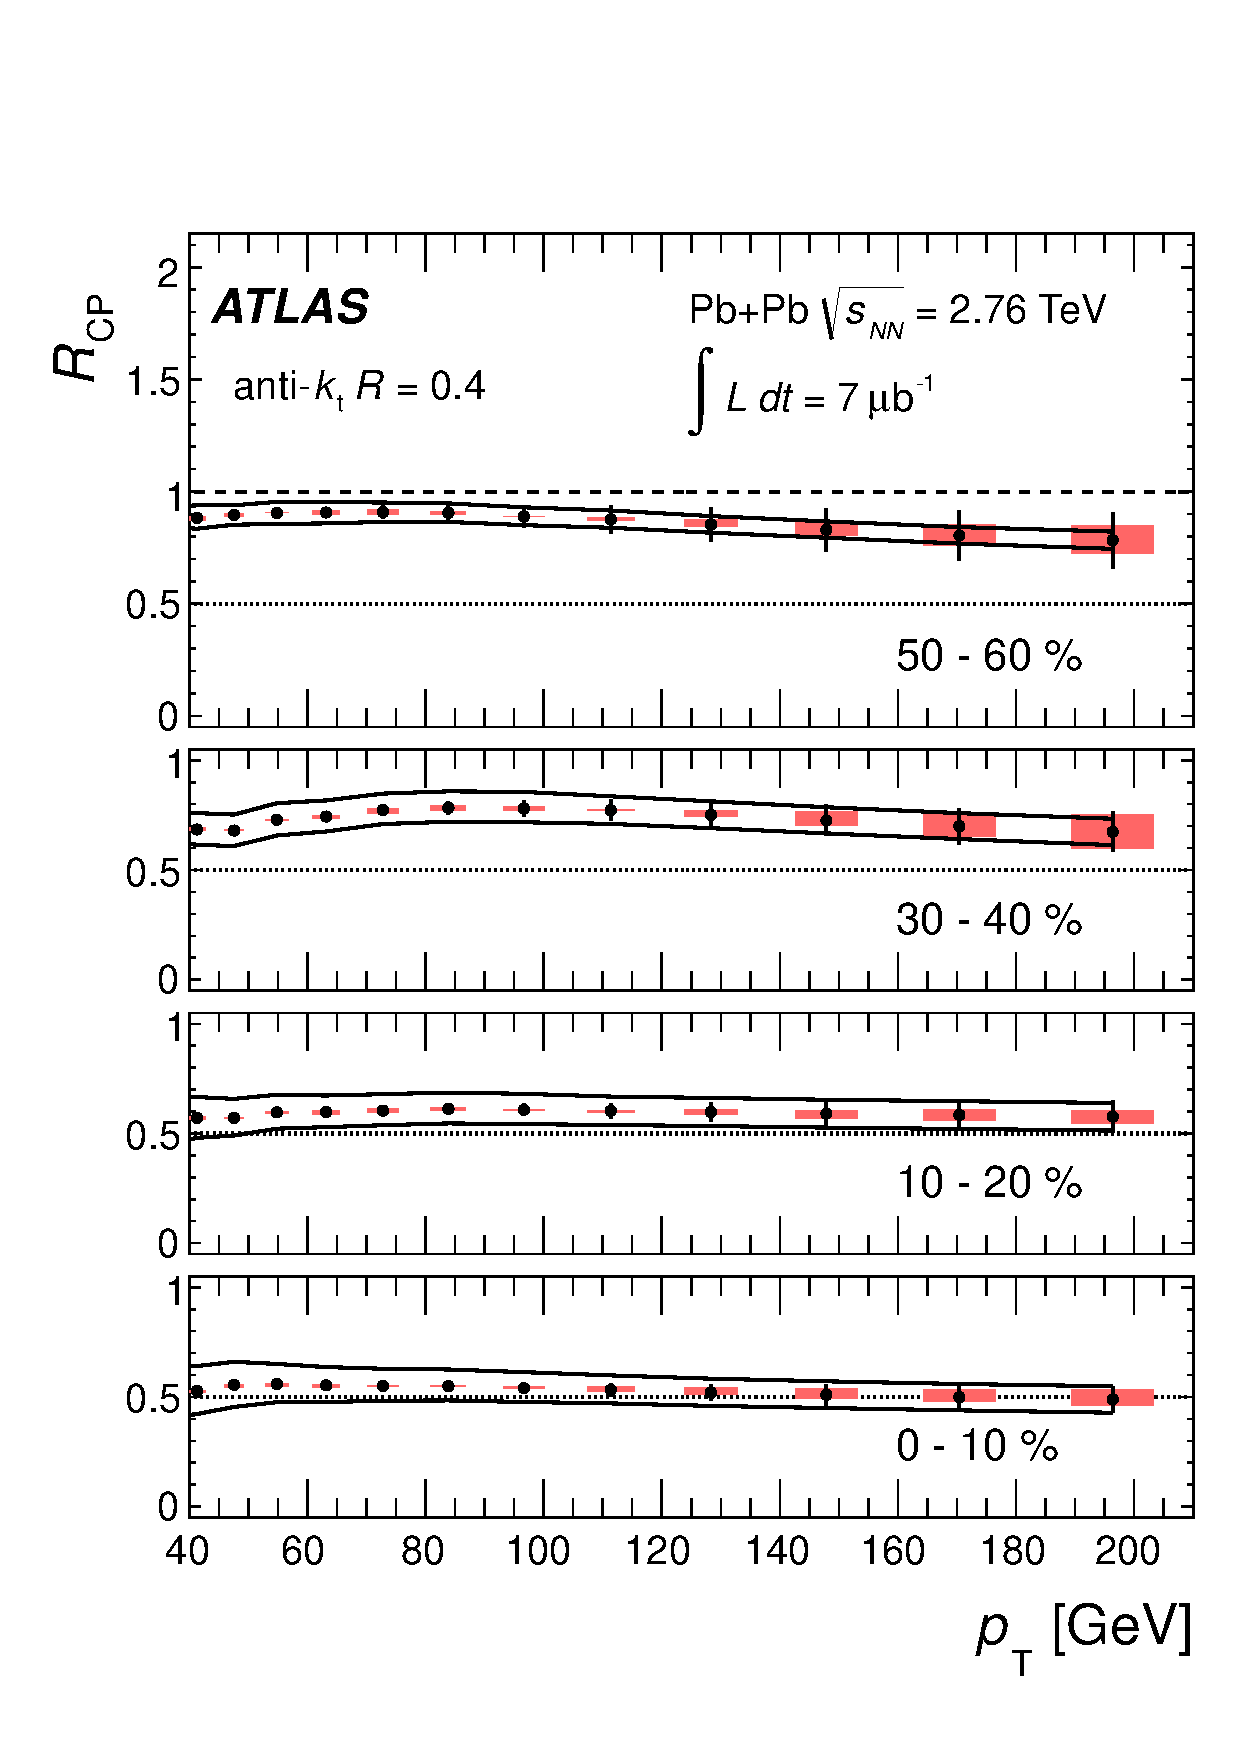
\includegraphics[width=0.4\textwidth]{jetfigures/ATLAS_jetRCP_04.pdf}
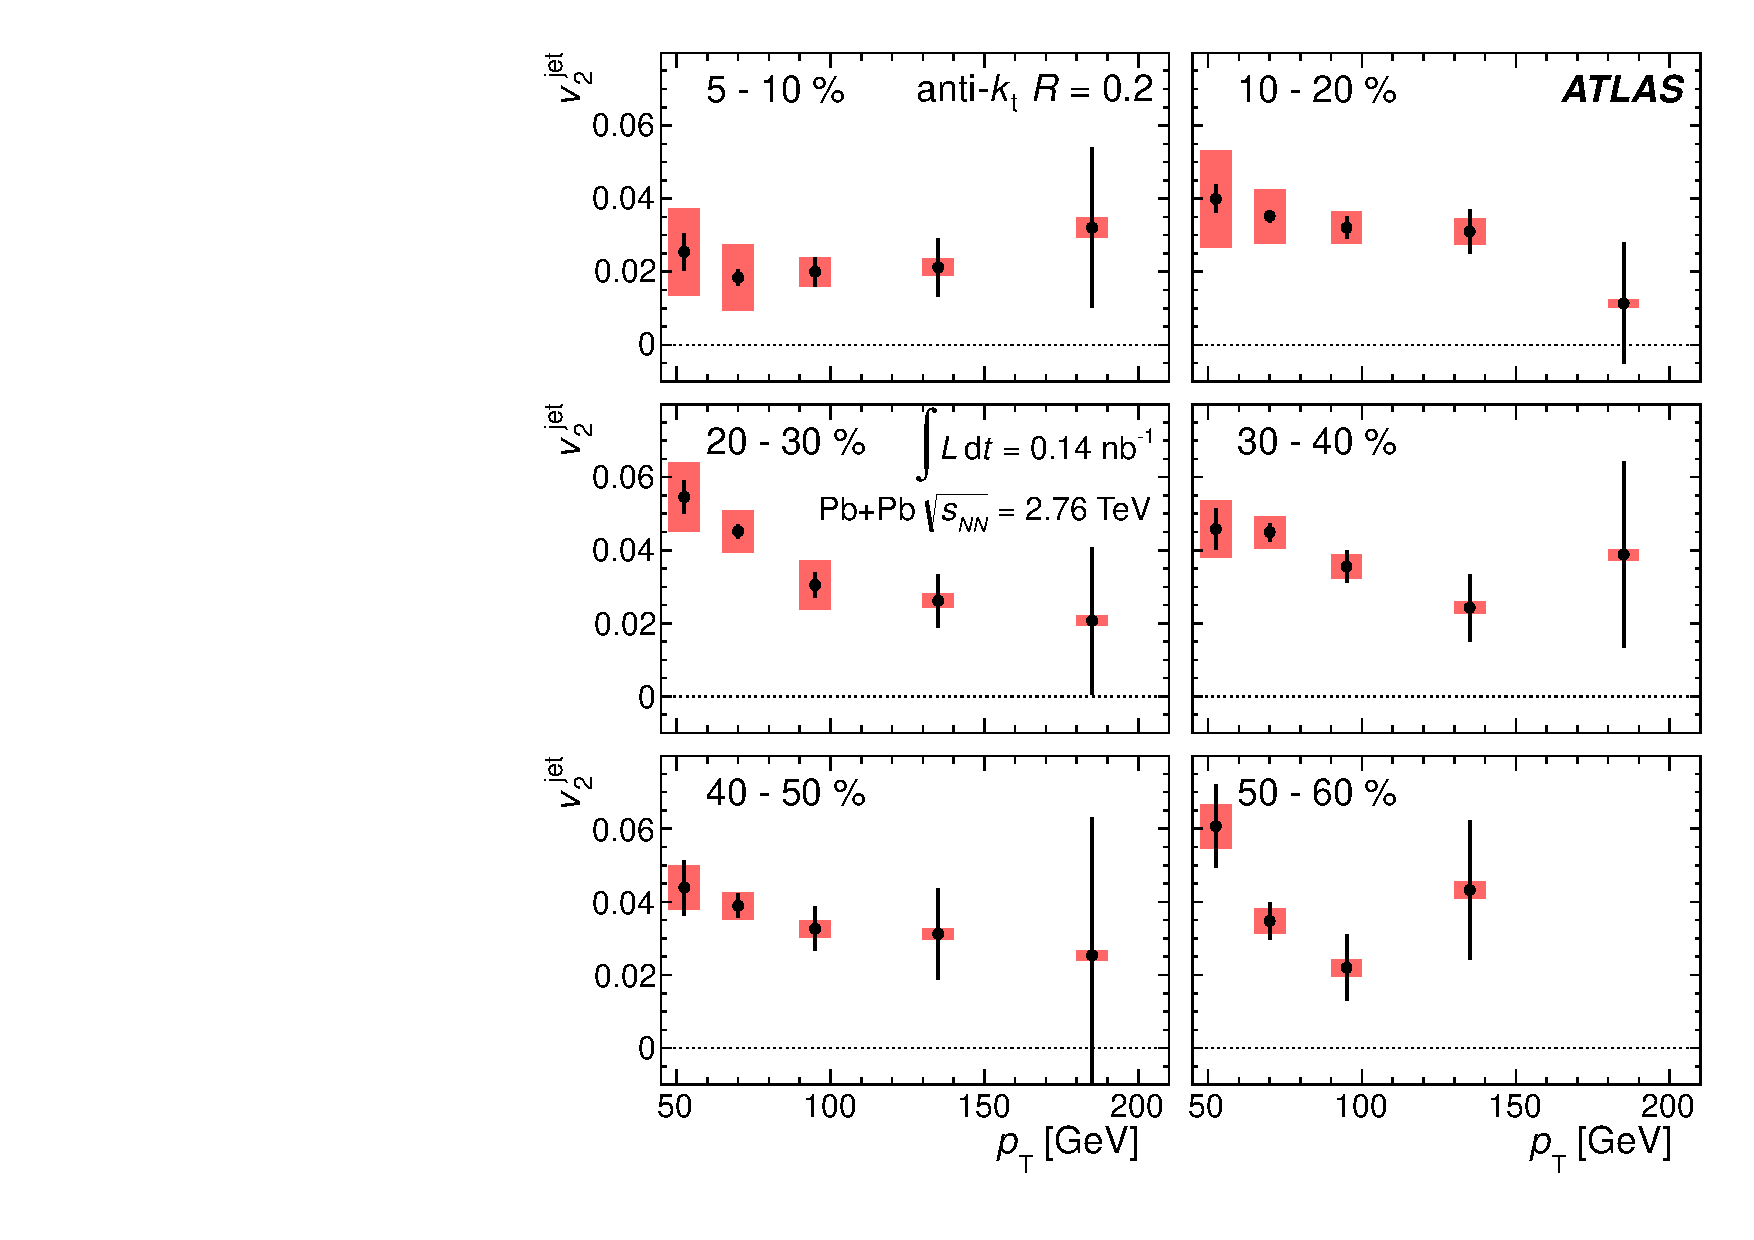
\includegraphics[width=0.49\textwidth]{jetfigures/ATLAS_jetv2.pdf}
\caption{
(left)\pT\ dependence of jet \Rcp\ for  $R=0.4$ jets,
in four bins of collision centrality. Error bars indicate
statistical errors while shaded boxes indicate
partially correlated systematic uncertainties. 
The solid lines show fully correlated uncertainties. 
Reproduced from~\cite{Aad:2012is}.
(right)\vtjet\ as a function of jet \pT\ in six bins of 
collision centrality.
Error bars indicate statistical uncertainties and 
systematic uncertainties are shown as shaded boxes. Reproduced from~\cite{Aad:2013sla}
}
\label{fig:pas:rcprfour}
\end{center}
\end{figure}

\subsection{Jet structure}

The study of both single and dijet jet rates clearly indicates that jets emitted in heavy ion 
collisions lose energy as they traverse the hot and dense medium.  It is natural to expect
that the radiation pattern emitted within a jet should be modified by the energy loss
process.  This has been addressed by a variety of approaches.

ATLAS has also measured the change in $R_{CP}$ as a function of jet radius (from 0.2 to 0.5) at
a fixed measured jet $\pT$.%  This is shown in Figure~\ref{fig:pas:ATLAS_jet_rcp}, where 
It is observed that the measured value of $R_{CP}$ increases significantly with increasing radius.
This indicates that jets with larger radius are slightly less suppressed, presumably since 
the jet energy profile is slightly wider in more central events.
%\begin{figure}[!th]
%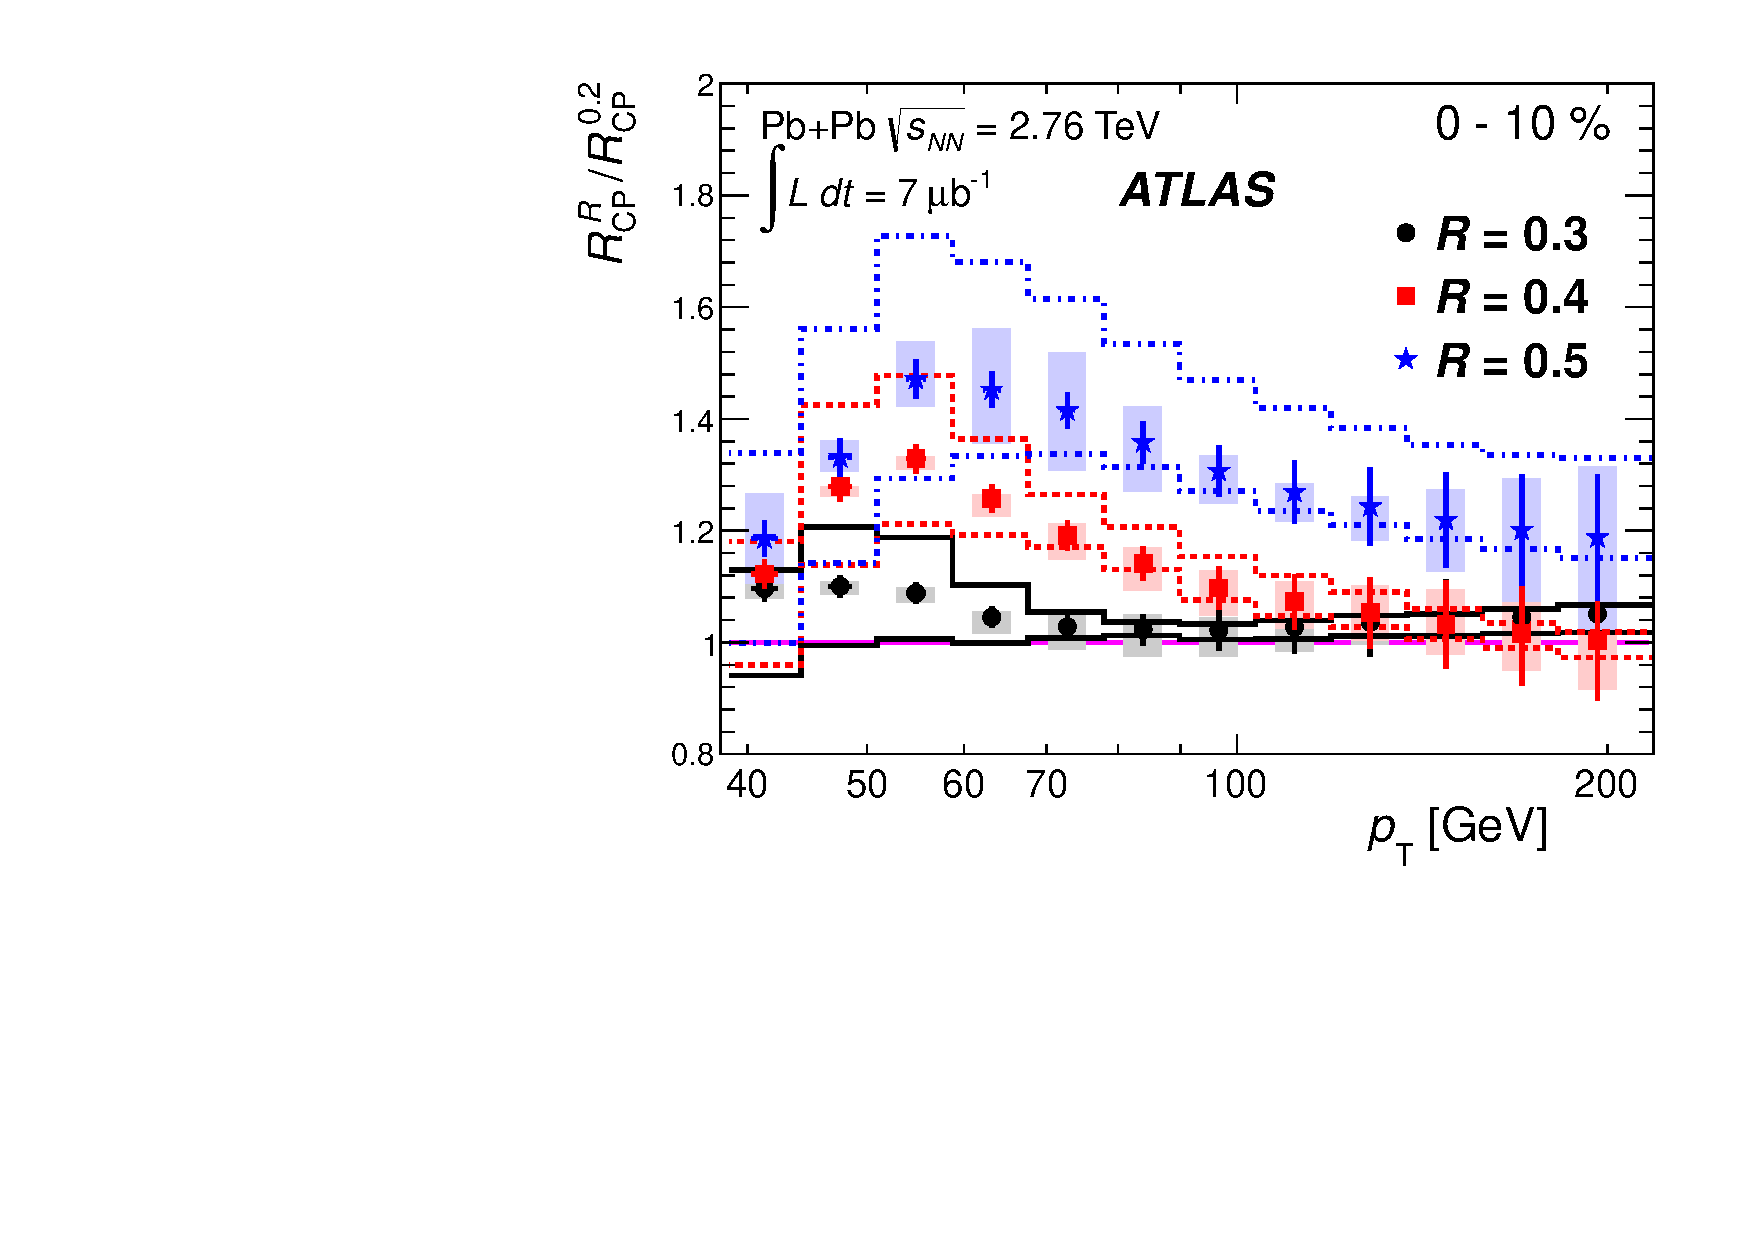
\includegraphics[width=0.59\textwidth]{jetfigures/ATLAS_jetRCP_size.pdf}
%\begin{center}
%\caption{
%Ratios of \Rcp\ values between $R = 0.3, 0.4$ and 0.5 jets and $R =
%0.2$ jets as a function of \pT\ in the 0--10\% centrality bin. The
%error bars show statistical uncertainties. The shaded boxes
%indicate partially correlated systematic errors. The lines indicate
%systematic errors that are fully correlated between different \pT\ bins.
%Reproduced from~\cite{Aad:2012is}.
%}
%\label{fig:pas:ATLAS_jet_rcp}
%\end{center}
%\end{figure}
%
The jet shape variable reflects the distribution of energy as a function of the radial coordinate
relative to the nominal jet direction.
The CMS measurements of jet shape as a function of centrality are shown in Figure~\ref{fig:pas:CMS_shape}.
The distributions for each system are individually normalized to unity.
The individual measurements in Pb+Pb and pp are shown as a function of centrality in the top row,
while their ratio is shown in the bottom row.
It is observed that the jet shape in peripheral collisions are consistent within uncertainties with pp,
while in the most central collisions, there is a depletion at moderate $r$ and an enhancment at large $r$.
While the relative enhancement at $r=0.3$ is large, it should be noted that the absolute change in the energy
flow is not large.

%The longitudinal fragmentation function $(1/N_{jet}) dN_{tr}/d\zeta$, where $\zeta = \ln(1/z)$ with
%$z = \p^{track}_{||}/p_{jet}$, measured in the dijet center-of-mass frame was 

\begin{figure}[!ht]
\begin{center}
%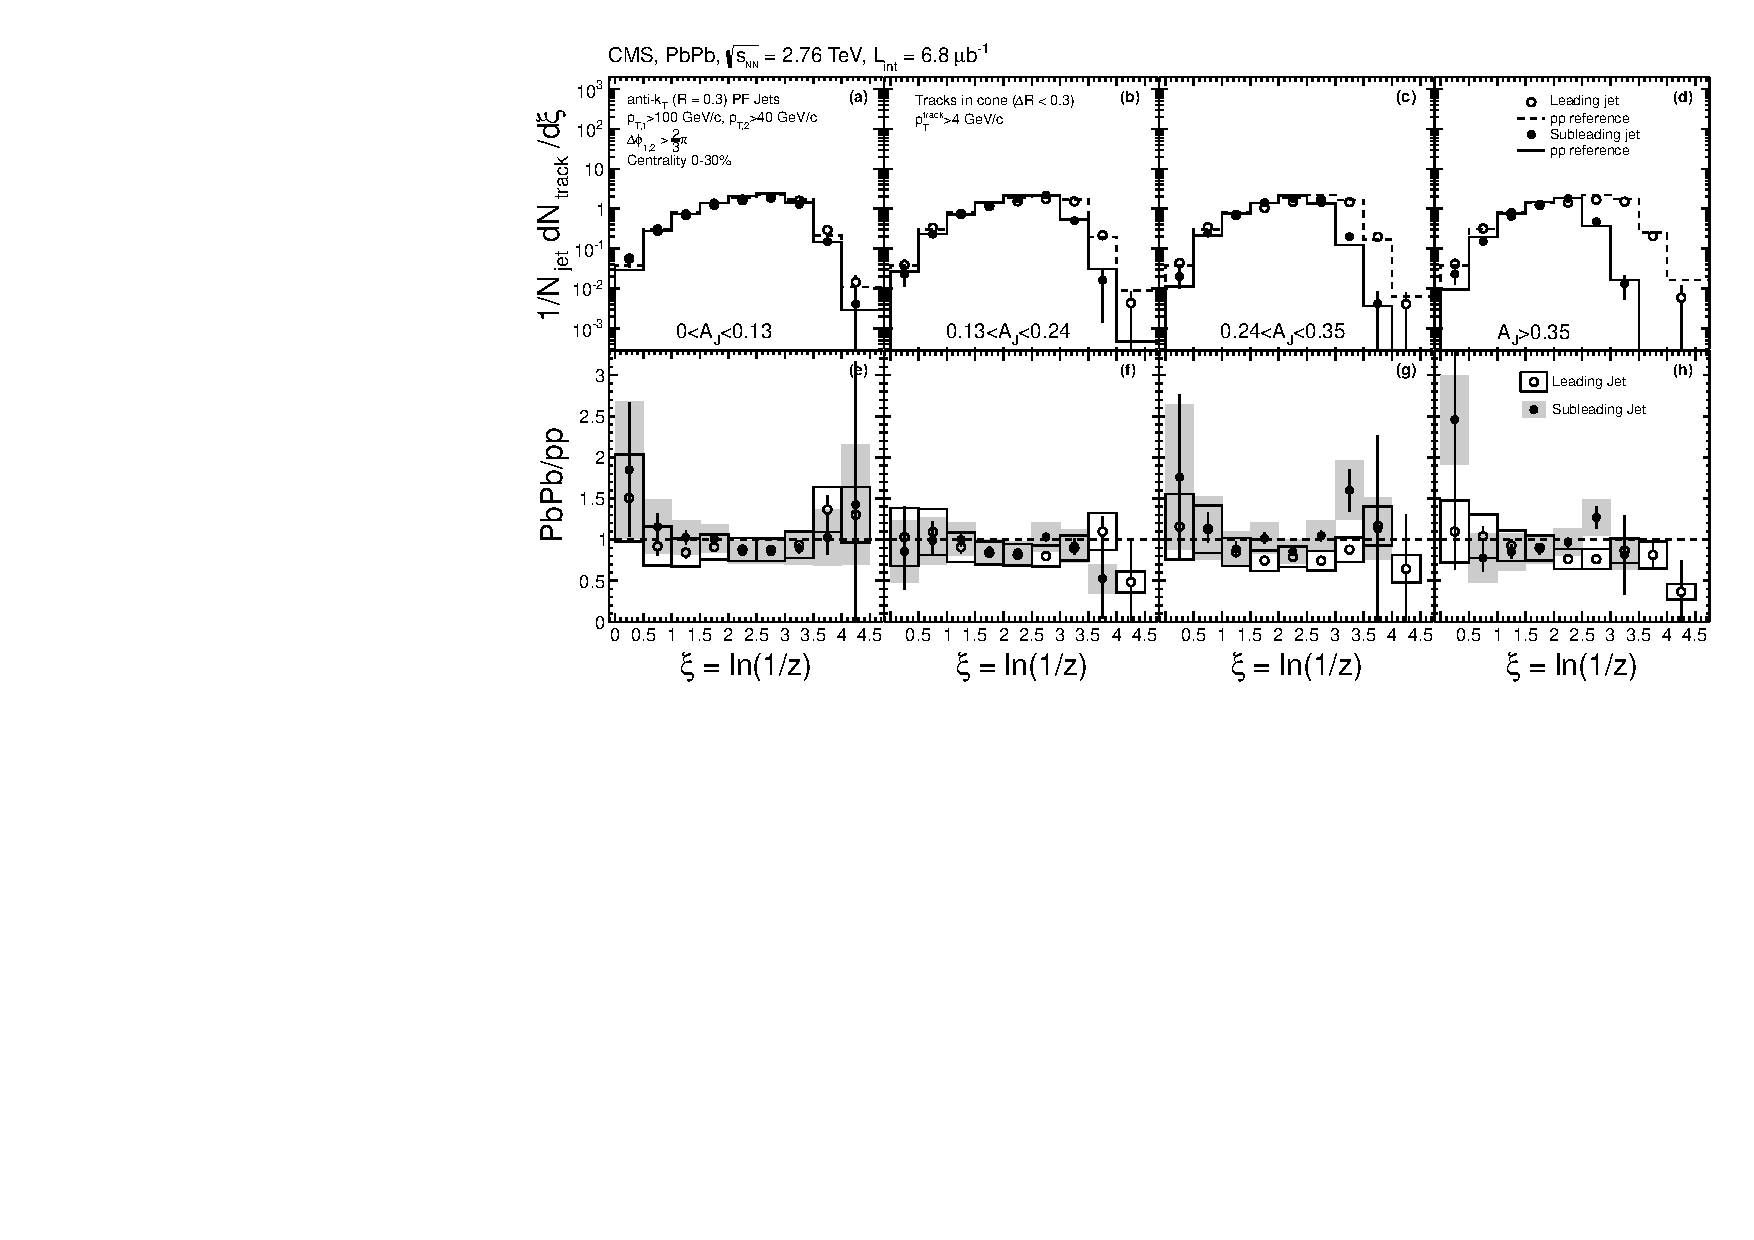
\includegraphics[width=0.8\textwidth]{jetfigures/xsi_div_both_effv9_l100s40_0to12_dphi20eta20dr3pt4id1_cwt_ppDiv_gray.pdf}
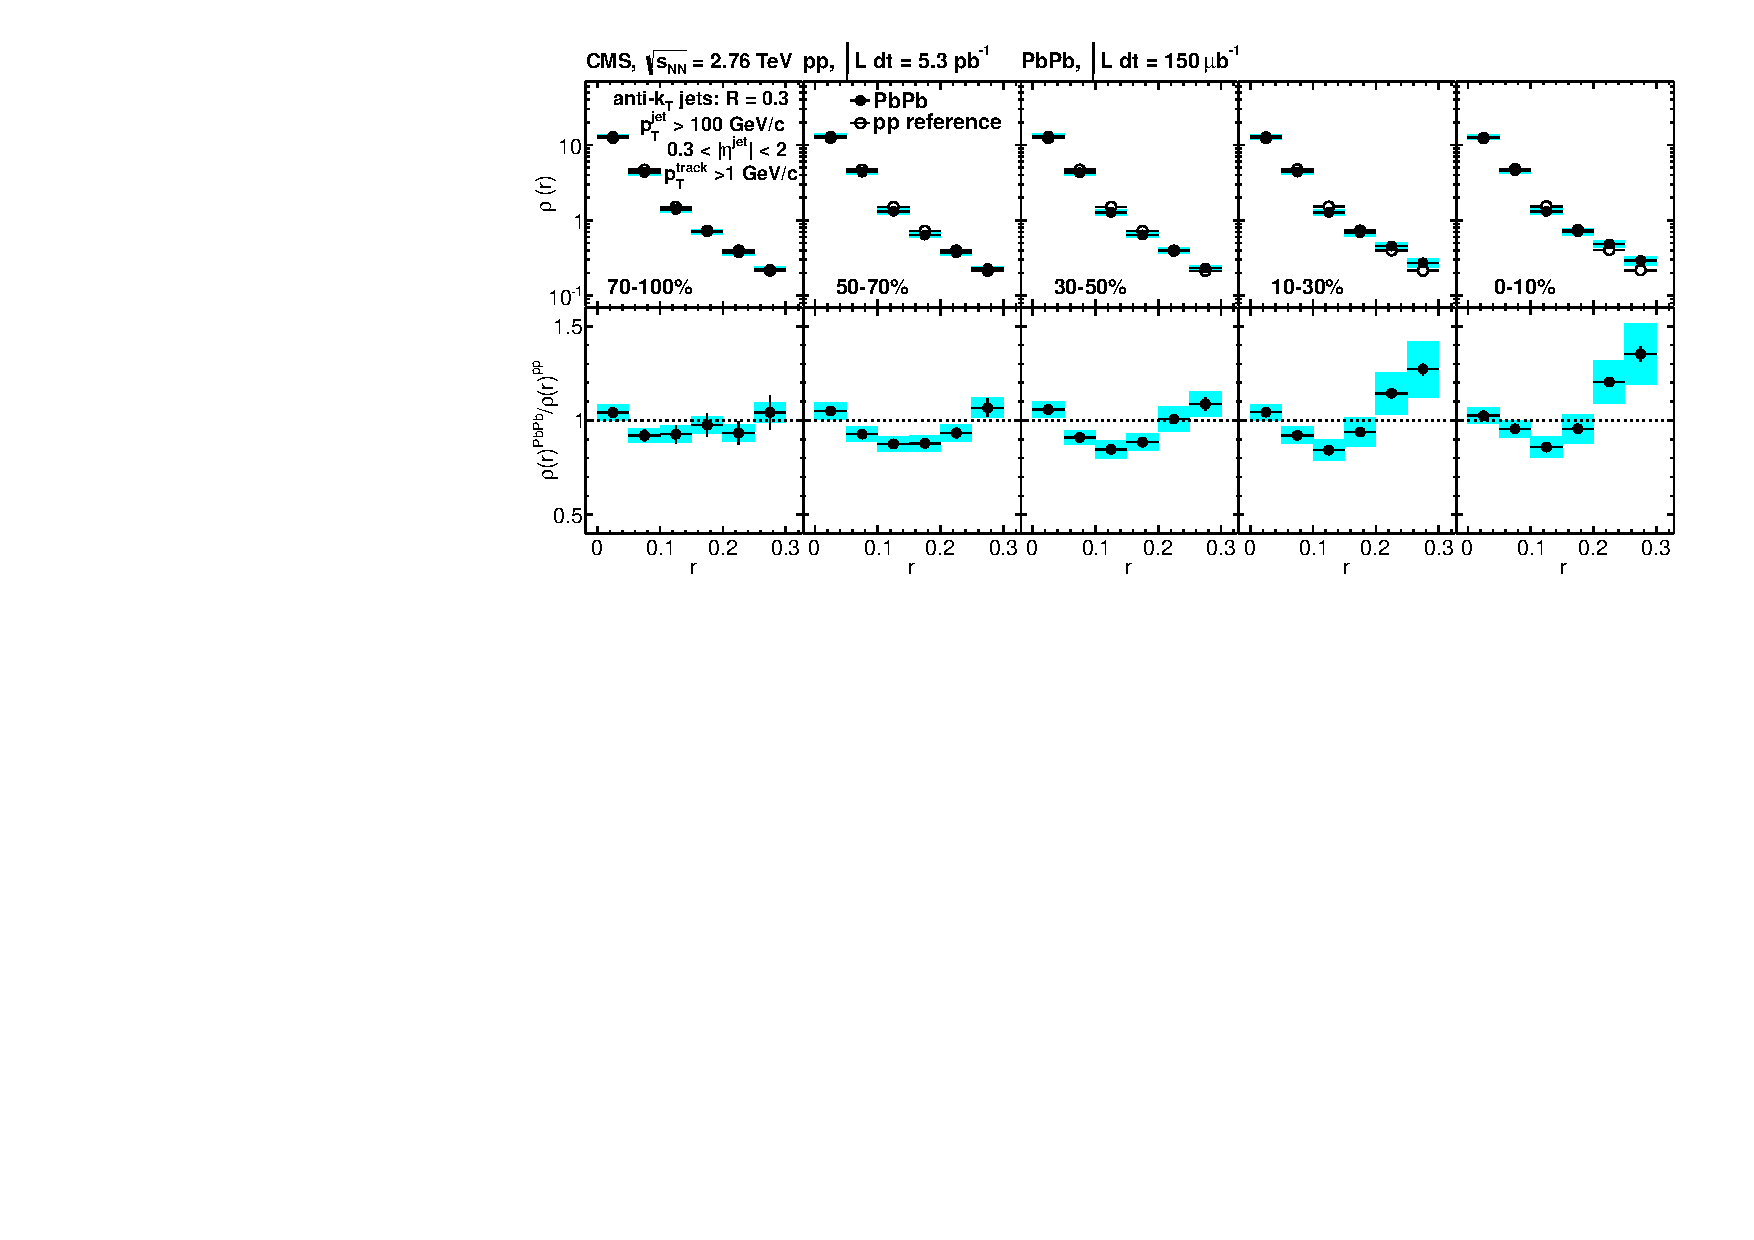
\includegraphics[width=0.8\textwidth]{jetfigures/cms_shape_Figure2.pdf}
\caption{
%(top)
%(a--d) Fragmentation functions for the leading (open circles) and subleading (solid points) 
%jets in four regions of $\AJ$ in central \PbPb\ collisions compared to the \pp\ reference.
%(e--h) Ratio of each fragmentation function to its \pp-based reference.
%Error bars shown are statistical. The systematic uncertainty is
%represented by hollow boxes (leading jet) or gray boxes (subleading jet).
%(i--l) Jet $\pT$ distributions in \PbPb\ collisions in four regions of $\AJ$
%compared to a \pp-based reference. Only statistical uncertainties are shown.
%Reproduced from~\cite{Chatrchyan:2012gw}.
%
(upper): Differential jet shapes in \PbPb\ collisions (filled circles)
as a function of distance from the jet axis for inclusive jets with $\pT^{\mbox{jet}} >100\GeVc$
in five bins of centrality.  The \pp-based reference is shown with open symbols.
The shaded regions represent the \PbPb\ systematic uncertainties.
Statistical uncertainties are smaller than the marker size.
(lower): Jet shape ratios $\rho(r)^{\PbPb}/\rho(r)^{\pp}$.
Error bars show the statistical uncertainties and shaded boxes indicate the systematic uncertainties. 
Reproduced from~\cite{Chatrchyan:2013kwa}
}
\label{fig:pas:CMS_shape}
\end{center}
\end{figure}

\subsection{Energy flow in dijet events}

The previous sections have demonstrated that the energy loss of jets is accompanied by a modest
change in jet structure within the nominal jet cone, suggestive of a broadening of the overall
jet energy flow.
Given this, it remains an open question where the rest of the lost energy goes.  
In the first CMS jet publication, the overall conservation of transverse momentum was used to 
study the energy flow associated with asymmetric dijets.  By using all tracks with $\pT>0.5$ GeV,
it was found that there was no missing transverse energy within the angular acceptance of the
CMS silicon tracker.  
The transverse energy balance was then compared in data and simulations 
for $\Delta R<0.8$ and $\Delta R >0.8$ as a function of the dijet asymmetry.
The most asymmetric events in the simulations achieved the overall energy balance 
with high momentum particles, suggesting that the balance at large angle was still achieved
by jet emission.  In the data, the energy balance was achieved by the emission of more 
soft particles, quite different than the simulations.

\begin{figure}[!ht]
\begin{center}
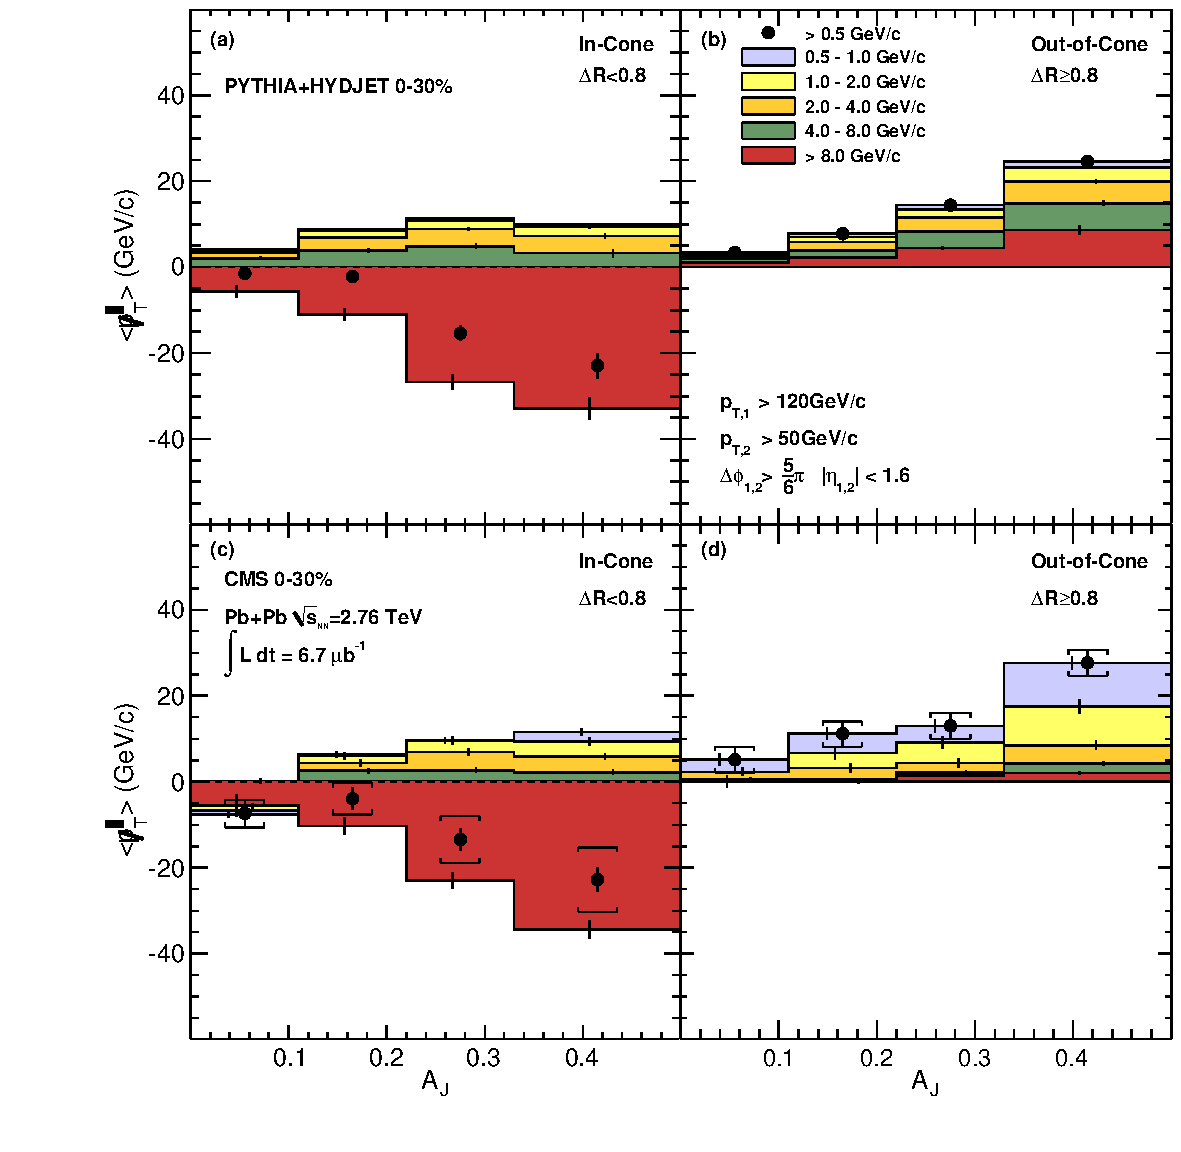
\includegraphics[width=0.5\textwidth]{jetfigures/missingPtParallel-Corrected-data-InConeOutConeDPhiCut_ntv6_2.pdf}
\caption{Average missing transverse momentum,
$\langle \displaystyle{\not} p_{\mathrm{T}}^{\parallel} \rangle$,
for tracks with $\pT > 0.5$\GeVc, projected onto the leading jet axis (solid circles).
The $\langle \displaystyle{\not} p_{\mathrm{T}}^{\parallel} \rangle$ values are
shown as a function of dijet asymmetry
$A_J$ for 0--30\% centrality, inside ($\Delta R < 0.8$) one of the leading or subleading jet cones (left) and
outside ($\Delta R > 0.8$) the leading and subleading jet cones (right).
For the solid circles, vertical bars and brackets represent
the statistical and systematic uncertainties, respectively.
For the individual $\pT$ ranges, the statistical uncertainties are shown as vertical bars.
Reproduced from~\cite{Chatrchyan:2011sx}.}
\label{fig:GR:CMS_missingpT}
\end{center}
\end{figure}

